\documentclass[a4paper]{article}
\usepackage[brazil]{babel}
\usepackage[utf8]{inputenc}
\usepackage[brazil]{babel}
\usepackage{multicol}
\usepackage{makeidx}
\usepackage{float}
\usepackage{array}
%\usepackage{a4wide}
\usepackage{boxedminipage}
\usepackage[dvipdfm]{hyperref}


 \usepackage[pdftex]{graphicx}
  % declare the path(s) where your graphic files are
   \graphicspath{{./pdf/}{./jpeg/}{./png/}}
  % and their extensions so you won't have to specify these with
  % every instance of \includegraphics
  \DeclareGraphicsExtensions{.pdf,.jpeg,.png}


%%%%%%%%%%%%%%%%%%%%%%%%%%%%%%%%%%%%%%%%%%%%%%%%%%%%%%%%%%%%%%%%%%%%%%%%%%%%%%%%

\makeindex
\title{Uma Aplicação no Google AppEngine}
\author{\textbf{Marcio Santos} ( Departamento)\\
        \textbf{Marcio Jose} ( Departamento )\\
        Taboca}
\def\latex/{\protect\LaTeX{}}
\newcommand{\bs}{\symbol{'134}}
\newcommand{\Cmd}[1]{\hspace{1em}\texttt{\def\{{\char`\{}\def\}{\char`\}}\bs#1}\ }
\newcommand{\CmdIndex}[1]{\index{#1@\texttt{\bs#1}}\Cmd{#1}\ }
\newcommand{\TTIndex}[1]{\index{#1@\texttt{#1}}\ }
\restylefloat{figure}
\renewcommand{\topfraction}{0.9}
\renewcommand{\bottomfraction}{0.9}
\renewcommand{\textfraction}{0.05}
\setlength{\parindent}{0pt}
\setlength{\parskip}{1ex}
\setlength{\emergencystretch}{4em}
\addtolength{\textheight}{-0.5in} % make it print better on US letter paper
\makeatletter
\renewcommand\l@section      {\@dottedtocline{1}{1.5em}{2.3em}}
\makeatother


%%%%%%%%%%%%%%%%%%%%%%%%%%%%%%%%%%%%%%%%%%%%%%%%%%%%%%%%%%%%%%%%%%%%%%%%%%%%%%%%

\begin{document}
\maketitle
\begin{abstract}
Este documento tem o objetivo de ensinar, em linguagem do tipo textual, ou estilo livro, o uso do sistema AppEngine. É importante que o usuário deste material esteja sempre ao lado do computador fazendo os exercícios. 
\end{abstract}
\tableofcontents


%%%%%%%%%%%%%%%%%%%%%%%%%%%%%%%%%%%%%%%%%%%%%%%%%%%%%%%%%%%%%%%%%%%%%%%%%%%%%%%%

\section{Introdu\c{c}\~{a}o}

AppEngine é uma tecnologia e também um serviço oferecido pelo Google. Neste sistema e serviço existem duas opções quanto a linguagem de programação. Uma opção é a linguagem Python ( Paiton ) e a outra opção é Java. Neste livro você estará utilizando a linguagem Python. Este livro encontra-se em desenvolvimento, assim é recomendado que você não seja um seguidor somente do livro. Se porventura entender que algo está faltando, por favor consulte outros autores ou simplesmente coloque o seu capítulo aqui também. O livro é divido em algumas partes. A primeira seção trata do básico, que é o SDK. Não é recomendado que o estudante pense que o SDK é parte de algo a se entender. Em geral o SDK e outros sistemas de auxílio são somente pequenas aplicações para facilitar a vida do profissional --- não se trata da aula em sí e não deve ser o foco maior do trabalho. O foco está em como utilizar a linguagem e como implementar soluções. Também é importante observar que o foco deve sempre estar em movimento e que não existe ponto final onde o estudante estará  pronto. O estudante está pronto no momento em  que ele faz a ação de aprender.

%%%%%%%%%%%%%%%%%%%%%%%%%%%%%%%%%%%%%%%%%%%%%%%%%%%%%%%%%%%%%%%%%%%%%%%%%%%%%%%%

\section{Ferramentas básicas}

\subsection{Editor de textos}

Faça download de um editor de textos que seja de código aberto e livre. Não é necessário que tenha cores mas esta é uma opção para o usuário. Se achar que é melhor cores, vá em frente, se achar outras opções interessantes, tudo bem também. Mas o editor de texto e outras ferramentas devem não ser o tópico maior do que está aprendendo. Estas são meras ferramentas para lhe auxiliar a entender. É importante evitar focar no aspecto que a ferramenta está fazendo coisas por você. Quem faz é você e não a ferramenta, ou seja, o entendimento do que fazer com quaisquer ferramentas é muito mais importante do que saber usar algumas ferramentas específicas e não saber o que fazer com outras similares. 

\subsection {Google AppEngine SDK} 

Faça download do Google AppEngine SDK. A documentação do SDK, no site do Google AppEngine ( Google por AppEngine ) deverá auxiliá-lo a fazer o download do SDK e possivelmente de outros requisitos. No caso, vamos trabalhar com a linguagem de programação Python, ou seja, você deverá fazer download do SDK AppEngine para Python. Uma vez que tiver este instalado, juntamente com possíveis requisitos que ele demandar, então volte para este manual. A figura  \ref{fig:appengine-sdk} mostra a tela de uma aplicação que vem com o SDK, o GoogleAppEngineLauncher. Observe que em geral um SDK contém um conjunto de ferramentas e também pode conter documentação. Esta aplicação executável é somente um pequeno componente que vem junto e que oferece algumas facilidades. De fato, no contexto do nosso manual, não utilizaremos esta interface mas utilizaremos a mesma funcionalidade, só que via o shell.


\begin{figure}[!h]
\centering
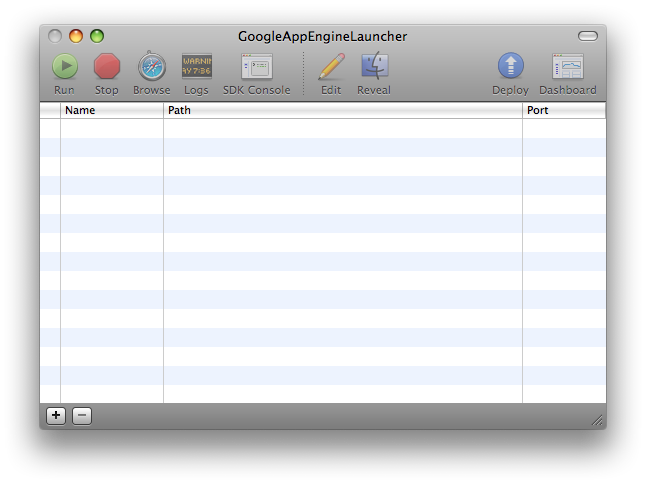
\includegraphics[width=4.4in]{image-appengine.png}
\caption{Screenshot de uma das aplicações que vem com o AppEngine SDK}
\label{fig:appengine-sdk}
\end{figure}.

Vale observar que o SDK, como uma ferramenta, também não é o foco do aprendizado. O SDK é muito simples e serve para testar a aplicação e também tem outros scripts que permitirão que você faça alguma manutenção. E, também,  possa enviar sua aplicação para a infra-estrutura de hosting(ou AppEngine cloud, da Google), no momento em que fizer o pedido, por meio de uma das aplicações-comando que vem com o SDK, que veremos em breve na seção Publicando Minha Primeira Aplicação. 

%%%%%%%%%%%%%%%%%%%%%%%%%%%%%%%%%%%%%%%%%%%%%%%%%%%%%%%%%%%%%%%%%%%%%%%%%%%%%%%%

\subsection{Shell - Linha de Comando e Atalhos do SDK}

Uma vez que o SDK for instalado você deverá testar se os atalhos estão funcionando, através de um shell - como o command.exe no caso do Windows, ou um xterm no Linux, ou a aplicação Terminal no Mac OS X. Abra uma janela de shell e chame o comando abaixo. A figura \ref{fig:appengine-sdk} mostra a tela de um usuário no Mac OS X logo após a execução do comando.  


\begin{verbatim}

dev_appserver.py

\end{verbatim}

Observe que esta aplicação-comando, do SDK, só irá executar caso ela esteja no PATH do seu shell. No caso do Mac OS X, o AppEngine SDK, durante a instalação, não coloca as aplicações do Google AppEngine SDK na variável de PATH dos usuários no shell. Se este for o seu caso, você deverá encontrar o local de instalação do Google App Engine SDK e adicionar o diretório no PATH ou mesmo executar o comando diretamente utilizando o path ( ou caminho ) completo. 


\begin{figure}[!h]
\centering
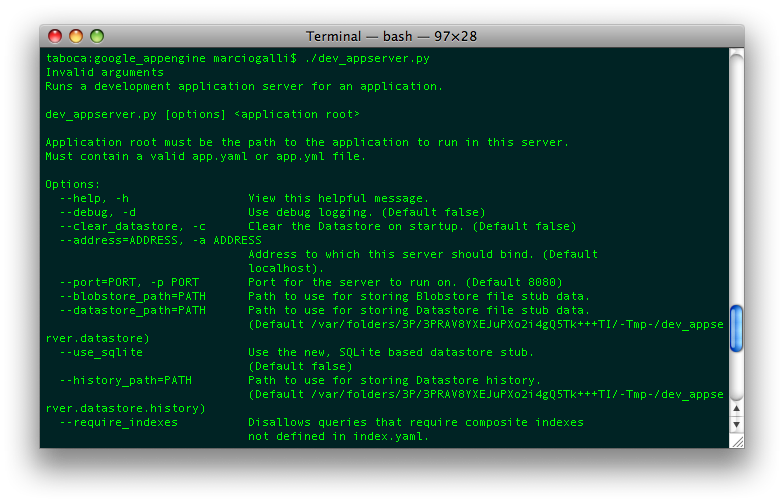
\includegraphics[width=5in]{image-dev_appserver.png}
\caption{Screenshot da tela do dev appserver}
\label{fig:appengine-sdk}
\end{figure}.

Uma vez que você sabe como executar esta aplicação você poderá tentar iniciar sua primeira aplicação. 

%%%%%%%%%%%%%%%%%%%%%%%%%%%%%%%%%%%%%%%%%%%%%%%%%%%%%%%%%%%%%%%%%%%%%%%%%%%%%%%%

\section{Primeira Aplicação}

Crie um diretório de trabalho em seu computador. Este diretório será o repositório de sua aplicação --- e conterá todos diversos arquivos como configuração, informações básicas para a infra estrutura Google AppEngine, arquivos de sua aplicação e também arquivos estáticos tipo HTML, CSS etc. É importante observar que o tipo de aplicação que o Google AppEngine faz é do tipo aplicação Web, ou seja, que é compatível com a arquitetura HTTP --- o modelo cliente-servidor. Se você não sabe o geral sobre o modelo cliente servidor então aproveite o valor da seção abaixo que oferece uma introdução. É importante ter o modelo cliente-servidor em mente pois irá facilitar o entendimento do que estaria rodando em um servidor versus o que roda no contexto do navegador. 

\begin{verbatim}

/meudiretorio/

\end{verbatim}

Utilizando um shell, faça o acesso a este diretório, ou seja, utilize do comando próprio do seu shell, seja ele Windows, Linux ou Mac OS, para "entrar no diretorio". É importante observar que em outros sistemas, como Windows, a estrutura de diretório pode ser um pouco diferente, mas, em geral, trata-se do mesmo tipo de estrutura de hierarquias que oferece suporte para a criação de arquivos e sub-diretórios. De dentro do diretório, certifique-se que você pode chamar as aplicações-comando que vem com o Google AppEngine SDK. Por exemplo a figura \ref{fig:image-shell-example} mostra um usuário tentando executar a aplicação-comando dev-appserver de dentro do diretorio minha-primeira-aplicacao: 

\begin{figure}[!h]
\centering
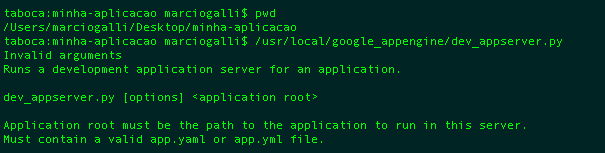
\includegraphics[width=5in]{image-shell-example.png}
\caption{Shell do usuário que executa um comando a partir de um novo diretório}
\label{fig:image-shell-example}
\end{figure}.


 

\subsection {Aplicação Cliente-Servidor via HTTP} 

O modelo para aplicações cliente-servidor HTTP é uma solução que permite que aplicações de software possam ser feitas ao mesmo tempo que garante compatibilidade com a solução Web de acesso as páginas HTML. É muito importante ter a noção completa sobre como que o navegador faz acesso ao servidor Web e então posteriormente entenderemos como a aplicação AppEngine tem um modelo baseado nesta arquitetura e como ela serve as páginas para o navegador e garante a sessão do usuário.  

Quando um usuário digita um URL como http://www.meusite.com o navegador faz uma conexão com o servidor disponibilizado em www.meusite.com utilizando uma porta tradicional, a porta 80. Quando o endereço URL não tem um PATH adicional, ou seja, não possui dados depois de uma barra no final ( tipo http://www.site.com/outros dados ) então o navegador irá pedir o documento "/" barra. O servidor de Web, que encontra-se no domínio do servidor ( meusite.com ) irá então responder com o documento que foi configurado como sendo o "/", em geral poderá servir um index.html. Uma vez que o servidor envia para o navegador o arquivo index.html ( vamos imaginar que neste servidor o / é um index.html ) a conexão é terminada. É muito importante observar que uma conexão foi criada por tempo determinado até que o pedido foi feito. Uma vez que a conexão é terminada o usuário pode ficar quanto tempo quiser visitando a página "/". 

Observe que na visão do usuário o conceito de página as vezes pode ser confuso. Neste caso o usuário tem a sensação que está visitando a "home" do site. Muitas vezes o usuário não tem a noção que "http://www.meusite.com" refere-se ao contexto PATH "/" no servidor, ou seja, que é o mesmo de acessar "http://www.meusite.com/". Em outras palavras, quando um usuário digita somente meusite.com, o browser que adiciona o "/" no final de maneira transparente. A figura \ref{fig:image-cliente-servidor} apresenta uma visão geral deste modelo onde o acesso a uma certa página HTML é de fato um processo que envolve um pedido ( requisição ) e que tem um retorno, uma conexão que tem inicio e fim. 


\begin{figure}[!h]
\centering
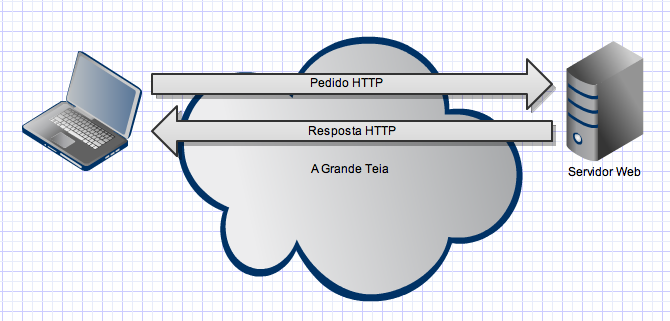
\includegraphics[width=4.5in]{image-cliente-servidor.png}
\caption{Usuário digita http://meusite.com/ e um pedido vai até o servidor que retorna uma página e a conexão então morre. }
\label{fig:image-cliente-servidor}
\end{figure}.

\subsection { HTML e HTTP e separação das requisições } 

Esta seção tem o objetivo de deixar mais evidente que as requisições do modelo HTTP, que é o protocolo de comunicação na Web, são temporárias --- elas deixam de existir assim que uma página chega ao navegador. Vamos imaginar o caso onde você está em um site que tem uma lista de items para outros documentos. Você então acesso primeiramente o http://www.meusite.com/ que é a página principal, ou home page, do site. Daí encontrou alguns links que dizem Link A, Link B, Link C. Estes três links ligam para outras páginas no mesmo servidor. No lado do servidor, no computador que encontra-se por exemplo em outra localização na Internet, tem-se os arquivos no sistema de arquivos: 

\begin{verbatim} 
/index.html  
/link-a.html
/link-b.html
/link-c.html
\end{verbatim} 

O usuário iniciou a sessão quando requisitou ao browser o endereço http://www.meusite.com/. Assim que o servidor recebe a requisição, este ( por estar previamente configurado para fazer uma regra ) devolveu a página index.html. Quando a página HTML chegou ao browser ele apresenta ao usuário --- a conexão HTTP morre no momento que a página chegou no browser. Se a página ( index.html ) tem links para Link A, Link B e Link C, então o usuário tem opção de acessar estas outras páginas. Vale notar que uma vez que a conexão HTTP não mais existe, o usuário pode ficar quando tempo quiser nesta página index.html. Este é um dos benefícios do modelo HTTP. Enquanto o usuário encontra-se lendo uma página ( ou esperando que seja ) não existe nenhum custo para o lado do servidor. No momento que o usuário clicar em um link na página, é que o navegador vai novamente iniciar um processo de pedir uma requisição para o servidor assim novamente uma conexão HTTP é criada e irá viver por tempo determinado até que a página ( endereço do link clicado ) seja retornada ao browser.

Esta noção é muito importante e permite maior facilidade para se entender como os serviços ou aplicações na Web são feitos. No início não havia aplicações no servidor e era tudo estático.  Mas a necessidade de se criar soluções dinâmicas fez com que diversos desenvolvedores criassem soluções onde programas funcionem no servidor e que sejam associados com o servidor de Web.

A figura \ref{fig:image-servidor-web-app} mostra o cenário que um usuário, através do browser, faz uma requisição para uma "página" que não é estática ( por exemplo algo que vem de um banco de dados ). Assim que servidor de Web recebe a requisição ( por exemplo "http://www.meusite.com/atualizacao/" o servidor Web pode então estabelecer uma ponte, ou seja, uma outra requisição para uma aplicação na mesma máquina servidor, que então deverá gerar uma página HTML, que será entregue de volta para o servidor Web, que irá devolver para browser. Em geral o usuário não tem como saber se uma dada página é de fato estática ( um HTML escrito uma vez ) ou dinâmica ( um HTML que foi gerado por um programa de computador ). 

\begin{figure}[!h]
\centering
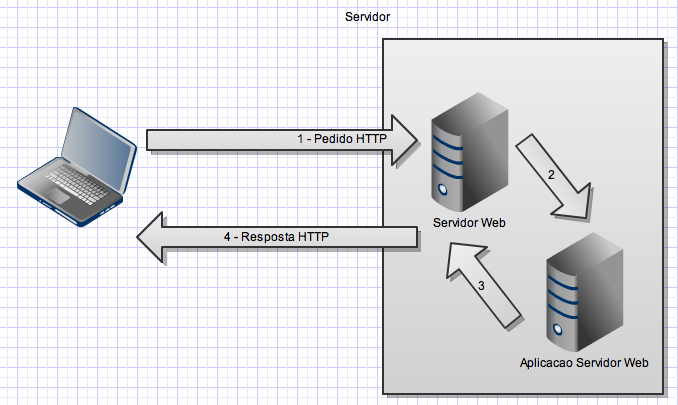
\includegraphics[width=4.5in]{image-servidor-web-app}
\caption{Cliente pede, servidor Web faz a ponte para Aplicação, volta pelo Servidor }
\label{fig:image-servidor-web-app}
\end{figure}.


\subsection {Dev AppServer Cria como um Servidor Web } 

Algo bem interessante que o Google AppEngine SDK faz é oferecer um pequeno servidor de Web que funciona no seu próprio computador. Este servidor tem grande parte da funcionalidade da infra-estrutura/servidor que o Google AppEngine oferece nos servidores Google. Este modelo permite que você possa testar grande parte da funcionalidade da sua aplicação de modo mais rápido, ou até de maneira offline. Uma vez que você acha que sua aplicação está rodando, mesmo que parcialmente, você pode então utilizar uma outra aplicação-ferramenta do AppEngine SDK e enviar a aplicação para o servidor Google utilizando suas credenciais.

O nosso primeiro exemplo será uma página HTML estática. Este exemplo tem o objetivo de lhe reforçar como o modelo cliente-servidor funciona e como o Google AppEngine possui as capacidades básicas de um servidor Web também. Depois de trabalharmos com a versão páginas estáticas, nós vamos então começar a alterar os arquivos da sua aplicação e vamos inserir uma camada de aplicação, ou seja, fazer com que a parte que roda no servidor possa fazer certas operações que páginas estáticas não conseguem. 

\subsection {Aplicação no Servidor Servindo Páginas Estáticas} 


\subsection { Publicando Minha Primeira Página } 


\subsection {Aplicação no Servidor Servindo Páginas Dinâmicas} 


\subsection { Publicando Minha Primeira Aplicação } 



\subsection { Banco de Dados no AppEngine } 

O AppEngine utiliza da tecnologia chamada BigTable \cite{bigtable} que trata-se de um sistema de armazenamento para dados estruturados que foi criado para funcionar de maneira distribuída. Isto significa que você não precisa se preocupar com complexidades relacionadas com a distribuição além de ter benefícios diversos no sentido de performance e simplicidade. 

%%%%%%%%%%%%%%%%%%%%%%%%%%%%%%%%%%%%%%%%%%%%%%%%%%%%%%%%%%%%%%%%%%%%%%%%%%%%%%%%

\printindex


\bibliographystyle{abbrv}
\bibliography{bibliography}  % sigproc.bib is the name of the Bibliography in this case




\end{document}
